\documentclass[10pt]{article}

% Specify the margins and text size.
\setlength{\textwidth}{6.4in}
\setlength{\textheight}{9.5in}
\setlength{\oddsidemargin}{0pt}
\setlength{\evensidemargin}{0pt}
\setlength{\topmargin}{0pt}
\setlength{\hoffset}{.05in}
\setlength{\voffset}{-1in}

\setlength{\parskip}{5pt}
\setlength{\parindent}{0pt}

% Load some fonts and symbol packages
\usepackage{latexsym}
\usepackage{pifont}       % contains 'star' symbol for counterinsurgency handbook title
\usepackage{yfonts} 
\usepackage{amsmath}
\usepackage{amsfonts}

\usepackage{graphicx}     % actually, this is loaded by pstricks
\usepackage[T1]{fontenc}
\usepackage{ifthen}
\usepackage{pstricks,pst-grad,pst-text,pst-node,multido,pst-plot,calc,pst-3dplot}
%\usepackage[all]{xy}
%\usepackage{animate}

% The hyperref package inserts links into the pdf.
\definecolor{MyLinkColor}{rgb}{.1,.2,1}
\definecolor{MyCiteColor}{rgb}{.1,1,.2}
\definecolor{MyURLColor}{rgb}{.4,.4,.4}
\usepackage[backref=true,pagebackref=false,hyperindex,colorlinks=true,
  linkcolor=MyLinkColor,urlcolor=MyURLColor]{hyperref}


% The tweaklist package is something I found on the web.  It provides a simple interface
% for making changes to spacing used in the itemize and enumerate environments.  Comment
% this out if you don't care to use tweaklist.
\usepackage{tweaklist}
\renewcommand{\itemhook}{\setlength{\parskip}{2pt}\setlength{\parsep}%
{1pt}\setlength{\topsep}{0pt}\setlength{\itemsep}{0pt}}

\newcommand{\U}{\underline{\hspace{5pt}}}

\usepackage{listings}
\newcommand{\Z}{\hphantom{0}}

\begin{document}
\pagestyle{empty}
\lstset{language=R, showspaces=false, showstringspaces=false}

\href{http://www.shepherd.edu}{
\includegraphics[height=1.75cm]{logo-high-res.eps}}
\vspace{-1.69cm}

{\small
\begin{tabular}{cl}
& Math 314\\
& Statistics\\
\hspace{5.28in} & %19 October 2011
\end{tabular}
}
\setlength{\baselineskip}{1.05\baselineskip}

\begin{center}
\textbf{\large  Exam II}
\end{center}
No books, notes or electronic devices may be used on this exam.
\medskip

1. (35 points) In a certain class, midterm scores average out to 60 with an SD of 15, as do 
scores on the final.  The correlation between midterm scores and final scores is 
about~$0.50$.   

\hspace{20pt} a) Write down the equation for the regression line. %(10 points)
\vspace{1.0in}

\hspace{20pt} b) Sketch the regression line. %(5 points)
\vspace{1.25in}

\hspace{20pt} c) 
Estimate the average final exam score for students whose midterm scores were
75, 30 and 60. %(10 points)
\vspace{2.75in}

\hspace{20pt} d) Estimate the midterm score for a student who scored 90 on the final exam.
%(5 points)
\vfill
\eject
{\ }


%\#7 page 144 (word problem about correlation)
%\#8 page 155 (word problem about correlation)
2. (10 points) For women age 25 and over in the U.S. in 2005, the relationship between
age and educational level (years of schooling completed) can be summarized as
follows. 
\begin{align*}
\mbox{average age}         & \approx \mbox{50 years,}    & \mbox{SD} & \approx \mbox{16 years}\\[3pt]
\mbox{average education level}  & \approx \mbox{13.2 years,}  & \mbox{SD} & \approx \mbox{3.0 years,
   \hspace{15pt}} r\approx -0.2
\end{align*}

\hspace{20pt} a) True or false:  For women age 25 and older in the U.S. in 2005, older women tended 
to be less\vspace{-5pt}

\hspace{20pt} \hphantom{a) }  educated than younger ones.
\bigskip

\hspace{20pt} b) True or false, and explain:  as you get older, you become less educated.  
If this statement is false,\vspace{-4pt}

\hspace{20pt} \hphantom{a) }
what could account for the negative correlation?  
\vspace{2in}


3. A box has 4 blue and 3 white marbles.  Calculate the following probabilities 
(5 points each)

\hspace{10pt} a) Drawing two blue in a row (with replacement)
\vspace{.4in}

\hspace{10pt} b) Drawing three white in a row (without replacement)\
\vspace{0.4in}

\hspace{10pt} c) Drawing at least one blue out of the first three (without replacement)
\vspace{1in}

4. (10 points) Test scores on a certain exam average out to 75 with a standard 
deviation of 3.  One student scored 84.   Was that a very high score?  Moderately high?  
Or about average?  Justify your answer.
\vfill
\eject
{\ }


5. (15 points) 

\hspace{20pt} a) For a representative sample of cars, would the correlation between the
age of the car and its gasoline economy (miles per gallon) be positive or negative?  Explain
\vspace{1.5in}

\hspace{20pt} b ) The correlation between gasoline economy and income of owner turns out to 
be positive?  How do you account for this association?
\vspace{1.5in}


6. (15 points) Suppose that the regression line of $y$ on $x$ 
is \[y=\left(\frac{\sqrt{3}}{2}\right)\,\left(\frac{8}{\sqrt{3}}\right)\,(x-1)\] 
where $\mbox{mean}_x=1$, $\mbox{mean}_y=0$, $\mbox{SD}_x=\sqrt{3}$, $\mbox{SD}_y=8$
and $r=\sqrt{3}/2$.\vspace{3pt}

\hspace{20pt} a) Calculate the RMS error for regression 
$\mbox{RMS}=\mbox{SD}_y\,\sqrt{1-r^2}$.  What can you say about the RMS\vspace{-4pt}

\hspace{20pt}\hphantom{b) } for the SD line?
\vspace{1.6in}

\hspace{20pt} b) If $x=2$, then we expect 68\% of the $y$-values to be
between \ \underline{\hspace{60pt}} \ \ and \  \underline{\hspace{60pt}} \ .

\vfill
\eject

\pagestyle{empty}

\href{http://www.shepherd.edu}{
\includegraphics[height=1.75cm]{logo-high-res.eps}}
\vspace{-1.69cm}

{\small
\begin{tabular}{cl}
& Math 314\\
& Statistics\\
\hspace{5.28in} & %19 October 2011
\end{tabular}
}

\begin{center}
\textbf{\large  Exam II}
\end{center}
No books, notes or electronic devices may be used on this exam.
\medskip

1. (35 points) In a certain class, midterm scores average out to 70 with an SD of 15, as do 
scores on the final.  The correlation between midterm scores and final scores is 
about~$0.50$.   

\hspace{20pt} a) Write down the equation for the regression line. %(10 points)
\vspace{1.0in}

\hspace{20pt} b) Sketch the regression line. %(5 points)
\vspace{1.25in}

\hspace{20pt} c) 
Estimate the average final exam score for students whose midterm scores were
85, 40 and 70. %(10 points)
\vspace{2.75in}

\hspace{20pt} d) Estimate the midterm score for a student who scored 90 on the final exam.
%(5 points)
\vfill
\eject
{\ }


%\#7 page 144 (word problem about correlation)
%\#8 page 155 (word problem about correlation)
2. (15 points) 

\hspace{20pt} a) For a representative sample of cars, would the correlation between the
age of the car and its gasoline economy (miles per gallon) be positive or negative?  Explain
\vspace{1.75in}

\hspace{20pt} b ) The correlation between gasoline economy and income of owner turns out to 
be positive?  How do you account for this association?
\vspace{2in}

3. A box has 4 blue and 3 white marbles.  Calculate the following probabilities 
(5 points each)

\hspace{10pt} a) Drawing two white in a row (with replacement)
\vspace{.4in}

\hspace{10pt} b) Drawing three blue in a row (without replacement)
\vspace{0.4in}

\hspace{10pt} c) Drawing at least one white out of the first three (without replacement)
\vspace{1in}

4. (10 points) Test scores on a certain exam average out to 75 with a standard 
deviation of 3.  One student scored 84.   Was that a very high score?  Moderately high?  
Or about average?  Justify your answer.
\vfill
\eject
{\ }
5. (10 points) For women age 25 and over in the U.S. in 2005, the relationship between
age and educational level (years of schooling completed) can be summarized as
follows. 
\begin{align*}
\mbox{average age}         & \approx \mbox{50 years,}    & \mbox{SD} & \approx \mbox{16 years}\\[3pt]
\mbox{average education level}  & \approx \mbox{13.2 years,}  & \mbox{SD} & \approx \mbox{3.0 years,
   \hspace{15pt}} r\approx -0.2
\end{align*}

\hspace{20pt} a) True or false:  For women age 25 and older in the U.S. in 2005, older women tended 
to be less\vspace{-5pt}

\hspace{20pt} \hphantom{a) }  educated than younger ones.
\bigskip

\hspace{20pt} b) True or false, and explain:  as you get older, you become less educated.  
If this statement is false,\vspace{-4pt}

\hspace{20pt} \hphantom{a) }
what could account for the negative correlation?  
\vspace{2in}


6. (15 points) Suppose that the regression line of $y$ on $x$ 
is \[y=\left(\frac{\sqrt{3}}{2}\right)\,\left(\frac{8}{\sqrt{3}}\right)\,(x-1)\] 
where $\mbox{mean}_x=1$, $\mbox{mean}_y=0$, $\mbox{SD}_x=\sqrt{3}$, $\mbox{SD}_y=8$
and $r=\sqrt{3}/2$.\vspace{3pt}

\hspace{20pt} a) Calculate the RMS error for regression 
$\mbox{RMS}=\mbox{SD}_y\,\sqrt{1-r^2}$.  What can you say about the RMS\vspace{-4pt}

\hspace{20pt}\hphantom{b) } for the SD line?
\vspace{2in}

\hspace{20pt} b) If $x=4$, then we expect 95\% of the $y$-values to be
between \ \underline{\hspace{60pt}} \ \ and \  \underline{\hspace{60pt}} \ .
\vspace{2in}



\vfill
\eject

{\ }
\vfill
\eject

\href{http://www.shepherd.edu}{
\includegraphics[height=1.75cm]{logo-high-res.eps}}
\vspace{-1.69cm}

{\small
\begin{tabular}{cl}
& Math 314\\
& Statistics\\
\hspace{5.28in} & %19 October 2011
\end{tabular}
}
\setlength{\baselineskip}{1.05\baselineskip}

\begin{center}
\textbf{\large  Exam II}
\end{center}
No books, notes or electronic devices may be used on this exam.
\medskip

1. (35 points) In a certain class, midterm scores average out to 60 with an SD of 15, as do 
scores on the final.  The correlation between midterm scores and final scores is 
about~$0.50$.   

\hspace{20pt} a) Write down the equation for the regression line. %(10 points)
\vspace{1.0in}

\hspace{20pt} b) Sketch the regression line. %(5 points)
\vspace{1.25in}

\hspace{20pt} c) 
Estimate the average final exam score for students whose midterm scores were
75, 30 and 60. %(10 points)
\vspace{2.75in}

\hspace{20pt} d) Estimate the midterm score for a student who scored 90 on the final exam.
%(5 points)
\vfill
\eject
{\ }


%\#7 page 144 (word problem about correlation)
%\#8 page 155 (word problem about correlation)
2. (10 points) For women age 25 and over in the U.S. in 2005, the relationship between
age and educational level (years of schooling completed) can be summarized as
follows. 
\begin{align*}
\mbox{average age}         & \approx \mbox{50 years,}    & \mbox{SD} & \approx \mbox{16 years}\\[3pt]
\mbox{average education level}  & \approx \mbox{13.2 years,}  & \mbox{SD} & \approx \mbox{3.0 years,
   \hspace{15pt}} r\approx -0.2
\end{align*}

\hspace{20pt} a) True or false:  For women age 25 and older in the U.S. in 2005, older women tended 
to be less\vspace{-5pt}

\hspace{20pt} \hphantom{a) }  educated than younger ones.
\bigskip

\hspace{20pt} b) True or false, and explain:  as you get older, you become less educated.  
If this statement is false,\vspace{-4pt}

\hspace{20pt} \hphantom{a) }
what could account for the negative correlation?  
\vspace{2in}


3. (15 points)
For the data given below, \vspace{-8pt}
\begin{center}
\begin{tabular}{llll}
x: & average $\approx 100$, & $\mbox{SD}\approx 12$\\
y: & average $\approx 110$, & $\mbox{SD}\approx 20$,  & $r\approx 0.6$\\
\end{tabular}\vspace{-8pt}
\end{center}
the equation for the regression line is $y=x+10$ and the RMS is $0.8$.
If $x=112$, then 68\% of the $y$-values are in what range?
\vspace{1.8in}


4. (15 points) Test scores on a certain exam average out to 75 with a standard 
deviation of 3.  One student scored 84.   Was that a very high score?  Moderately high?  
Or about average?  Justify your answer.
\vfill
\eject
{\ }


5. (15 points) 

\hspace{20pt} a) For a representative sample of cars, would the correlation between the
age of the car and its gasoline economy (miles per gallon) be positive or negative?  Explain
\vspace{1.5in}

\hspace{20pt} b ) The correlation between gasoline economy and income of owner turns out to 
be positive?  How do you account for this association?
\vspace{1.5in}


6. (15 points) Suppose that the regression line of $y$ on $x$ 
is \[y=\left(\frac{\sqrt{3}}{2}\right)\,\left(\frac{8}{\sqrt{3}}\right)\,(x-1)\] 
where $\mbox{mean}_x=1$, $\mbox{mean}_y=0$, $\mbox{SD}_x=\sqrt{3}$, $\mbox{SD}_y=8$
and $r=\sqrt{3}/2$.\vspace{3pt}

\hspace{20pt} a) Calculate the RMS error for regression 
$\mbox{RMS}=\mbox{SD}_y\,\sqrt{1-r^2}$.  What can you say about the RMS\vspace{-4pt}

\hspace{20pt}\hphantom{b) } for the SD line?
\vspace{1.6in}

\hspace{20pt} b) If $x=2$, then we expect 95\% of the $y$-values to be
between \ \underline{\hspace{60pt}} \ \ and \  \underline{\hspace{60pt}} \ .

\vfill
\eject

\pagestyle{empty}

\href{http://www.shepherd.edu}{
\includegraphics[height=1.75cm]{logo-high-res.eps}}
\vspace{-1.69cm}

{\small
\begin{tabular}{cl}
& Math 314\\
& Statistics\\
\hspace{5.28in} & %19 October 2011
\end{tabular}
}

\begin{center}
\textbf{\large  Exam II}
\end{center}
No books, notes or electronic devices may be used on this exam.
\medskip

1. (35 points) In a certain class, midterm scores average out to 70 with an SD of 15, as do 
scores on the final.  The correlation between midterm scores and final scores is 
about~$0.50$.   

\hspace{20pt} a) Write down the equation for the regression line. %(10 points)
\vspace{1.0in}

\hspace{20pt} b) Sketch the regression line. %(5 points)
\vspace{1.25in}

\hspace{20pt} c) 
Estimate the average final exam score for students whose midterm scores were
85, 40 and 70. %(10 points)
\vspace{2.75in}

\hspace{20pt} d) Estimate the midterm score for a student who scored 90 on the final exam.
%(5 points)
\vfill
\eject
{\ }


%\#7 page 144 (word problem about correlation)
%\#8 page 155 (word problem about correlation)
2. (15 points) 

\hspace{20pt} a) For a representative sample of cars, would the correlation between the
age of the car and its gasoline economy (miles per gallon) be positive or negative?  Explain
\vspace{1.75in}

\hspace{20pt} b ) The correlation between gasoline economy and income of owner turns out to 
be positive?  How do you account for this association?
\vspace{2in}

3. (15 points)
For the data given below, \vspace{-8pt}
\begin{center}
\begin{tabular}{llll}
x: & average $\approx 100$, & $\mbox{SD}\approx 12$\\
y: & average $\approx 110$, & $\mbox{SD}\approx 20$,  & $r\approx 0.6$\\
\end{tabular}\vspace{-8pt}
\end{center}
the equation for the regression line is $y=x+10$ and the RMS is $0.8$.
If $x=80$, then 95\% of the $y$-values are in what range?
\vspace{1.8in}



4. (10 points) Test scores on a certain exam average out to 75 with a standard 
deviation of 3.  One student scored 84.   Was that a very high score?  Moderately high?  
Or about average?  Justify your answer.
\vfill
\eject
{\ }
5. (10 points) For women age 25 and over in the U.S. in 2005, the relationship between
age and educational level (years of schooling completed) can be summarized as
follows. 
\begin{align*}
\mbox{average age}         & \approx \mbox{50 years,}    & \mbox{SD} & \approx \mbox{16 years}\\[3pt]
\mbox{average education level}  & \approx \mbox{13.2 years,}  & \mbox{SD} & \approx \mbox{3.0 years,
   \hspace{15pt}} r\approx -0.2
\end{align*}

\hspace{20pt} a) True or false:  For women age 25 and older in the U.S. in 2005, older women tended 
to be less\vspace{-5pt}

\hspace{20pt} \hphantom{a) }  educated than younger ones.
\bigskip

\hspace{20pt} b) True or false, and explain:  as you get older, you become less educated.  
If this statement is false,\vspace{-4pt}

\hspace{20pt} \hphantom{a) }
what could account for the negative correlation?  
\vspace{2in}


6. (15 points) Suppose that the regression line of $y$ on $x$ 
is \[y=\left(\frac{\sqrt{3}}{2}\right)\,\left(\frac{8}{\sqrt{3}}\right)\,(x-1)\] 
where $\mbox{mean}_x=1$, $\mbox{mean}_y=0$, $\mbox{SD}_x=\sqrt{3}$, $\mbox{SD}_y=8$
and $r=\sqrt{3}/2$.\vspace{3pt}

\hspace{20pt} a) Calculate the RMS error for regression 
$\mbox{RMS}=\mbox{SD}_y\,\sqrt{1-r^2}$.  What can you say about the RMS\vspace{-4pt}

\hspace{20pt}\hphantom{b) } for the SD line?
\vspace{2in}

\hspace{20pt} b) If $x=4$, then we expect 68\% of the $y$-values to be
between \ \underline{\hspace{60pt}} \ \ and \  \underline{\hspace{60pt}} \ .
\vspace{2in}



\vfill
\eject

%%%%%%%%%%%%%%%%%%%%%%%%%%%%%%%%% HERE 
\pagestyle{empty}

\href{http://www.shepherd.edu}{
\includegraphics[height=1.75cm]{logo-high-res.eps}}
\vspace{-1.69cm}

{\small
\begin{tabular}{cl}
& Math 314\\
& Statistics\\
\hspace{5.28in} & %19 October 2011
\end{tabular}
}

\begin{center}
\textbf{\large  Exam II}
\end{center}
No books, notes or electronic devices may be used on this exam.
\medskip

1. (35 points)  The length of odontoblasts (tooth cells) in each of 10 guinea pigs 
at each of three dose levels of vitamin~C (0.5, 1, and 2 mg) 
is measured.  The scatter plot of the data is shown below.

\begin{center}
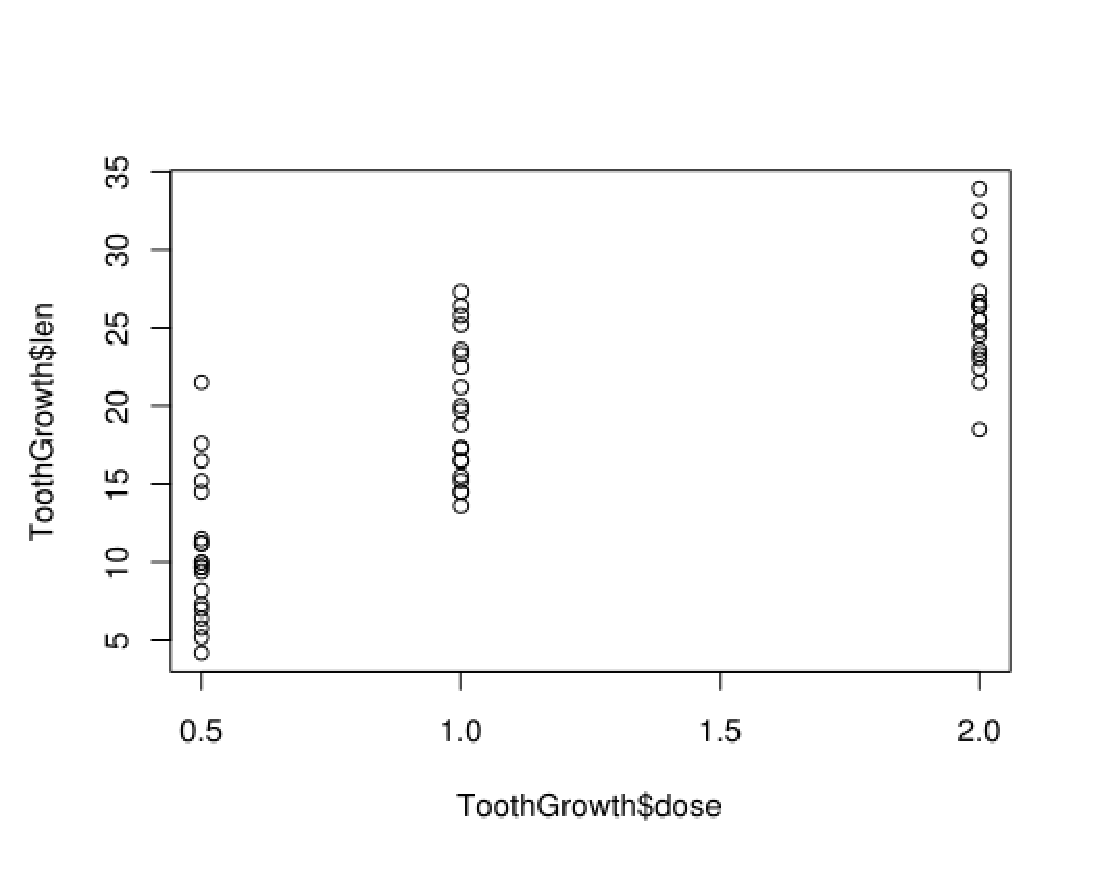
\includegraphics[height=1.75in,bb=0 22 515 340, clip]{teeth.eps}
\end{center}
The equation for the regression line computed from the data is 
\[y \approx 10\,x + 7\]
where $x$ is dose level in mg and $y$ is odontoblast length.
The correlation coefficient for the data is $r\approx 0.8$.

\hspace{20pt} a) Sketch the regression line in the above plot.
\medskip

\hspace{20pt} b) Estimate the odontoblast length for the dose levels $1.5$ mg, 2.0 mg and 2.5 mg.
\vspace{1.4in}

\hspace{20pt} c) The RMS error for the regression line is $4.5$.
Among guinea pigs that receive a vitamin C dose level of 1 mg, 68\% 
  have odontoblast length in what range?
\vspace{1.2in}

\hspace{20pt} d) One measurement has $\mbox{dose}=2.0$ mg and 
$\mbox{length}=23.0$. Calculate the length predicted by the regression
line then calculate the error (residual) for that value.

\vfill
\eject
{\ }


%\#7 page 144 (word problem about correlation)
%\#8 page 155 (word problem about correlation)
2. (15 points) 

\hspace{20pt} a) For a representative sample of cars, would the correlation between the
horsepower of the motor and  and its gasoline economy (miles per gallon) be positive or negative?  Explain
\vspace{1.75in}

\hspace{20pt} b ) The correlation between gasoline economy and age of the car turns out to 
be positive?  How do you account for this association?
\vspace{2in}

3. (15 points)
For the data given below, \vspace{-8pt}
\begin{center}
\begin{tabular}{llll}
x: & average $\approx 100$, & $\mbox{SD}\approx 12$\\
y: & average $\approx 110$, & $\mbox{SD}\approx 20$,  & $r\approx 0.6$\\
\end{tabular}\vspace{-8pt}
\end{center}
Write down the equation for the regression line to predict $y$ from $x$.
The RMS turns out to be 8.  
If $x=80$, then 95\% of the $y$-values are in what range?
\vspace{1.8in}



4. (10 points) Test scores on a certain exam average out to 75 with a standard 
deviation of 5.  One student scored 84.   Was that a very high score?  Moderately high?  
Or about average?  Justify your answer.
\vfill
\eject
{\ }
5. (10 points) 
For men age 25--34, the relationship between education (years of schooling
completed) and systolic blood pressure can be summarized as follows.
\begin{align*}
\mbox{average education} &\approx 13 \mbox{ years},
  & \mbox{SD} &\approx 3 \mbox{ years}\\
\mbox{average blood pressure} &\approx 119 \mbox{ mm}
  & \mbox{SD} &\approx 12 \mbox{ mm}
\end{align*}
The correlation coefficient is $r\approx -0.1$.

\hspace{20pt} a) True or false:  Men with higher education tended to have lower blood pressure.
\bigskip

\hspace{20pt} b) True or false, and explain:  Higher education causes lower blood pressure.
\vspace{2in}


6. (15 points) Suppose that the regression line of $y$ on $x$ 
is \[y=\left(\frac{\sqrt{3}}{2}\right)\,\left(\frac{8}{\sqrt{3}}\right)\,(x-1)\] 
where $\mbox{mean}_x=1$, $\mbox{mean}_y=0$, $\mbox{SD}_x=\sqrt{3}$, $\mbox{SD}_y=8$
and $r=\sqrt{3}/2$.\vspace{3pt}

\hspace{20pt} a) Calculate the RMS error for regression 
$\mbox{RMS}=\mbox{SD}_y\,\sqrt{1-r^2}$.  What can you say about the RMS\vspace{-4pt}

\hspace{20pt}\hphantom{b) } for the SD line?
\vspace{2in}

\hspace{20pt} b) If $x=4$, then we expect 68\% of the $y$-values to be
between \ \underline{\hspace{60pt}} \ \ and \  \underline{\hspace{60pt}} \ .
\vspace{2in}



\vfill
\eject





\end{document}

%%%%%%%%%%%%%%%%%%%%%%%%%%%%%%%%%%%%%%%%%%%%%%%%%%%%%%%%%%%%%%%%%%%%%%%%%%

\href{http://www.shepherd.edu}{
\includegraphics[height=1.75cm]{logo-high-res.eps}}
\vspace{-1.69cm}

{\small
\begin{tabular}{cl}
& Math 314\\
& Statistics\\
\hspace{5.28in} & 19 October 2011
\end{tabular}
}
\setlength{\baselineskip}{1.05\baselineskip}

\begin{center}
\textbf{\large  Exam II}
\end{center}
No books, notes or electronic devices may be used on this exam.
\medskip

1. (35 points) In a certain class, midterm scores average out to 70 with an SD of 12, as do 
scores on the final.  The correlation between midterm scores and final scores is 
about~$0.50$.   

\hspace{20pt} a) Sketch the regression line. %(5 points)
\vspace{1.25in}

\hspace{20pt} b) Write down the equation for the regression line. %(10 points)
\vspace{1in}

\hspace{20pt} c) 
Estimate the average final exam score for students whose midterm scores were
94, 58 and 70. %(10 points)
\vspace{2.75in}

\hspace{20pt} d) Estimate the midterm score for a student who scored 46 on the final exam.
%(5 points)
\vfill
\eject
{\ }


%\#7 page 144 (word problem about correlation)
%\#8 page 155 (word problem about correlation)
2. (10 points) For women age 25 and over in the U.S. in 2005, the relationship between
age and educational level (years of schooling completed) can be summarized as
follows. 
\begin{align*}
\mbox{average age}         & \approx \mbox{50 years,}    & \mbox{SD} & \approx \mbox{16 years}\\[3pt]
\mbox{average education level}  & \approx \mbox{13.2 years,}  & \mbox{SD} & \approx \mbox{3.0 years,
   \hspace{15pt}} r\approx -0.2
\end{align*}

\hspace{20pt} a) True or false:  For women age 25 and older in the U.S. in 2005, younger women tended 
to be more\vspace{-5pt}

\hspace{20pt} \hphantom{a) }  educated than older ones.
\bigskip

\hspace{20pt} b) True or false, and explain:  as you get older, you become less educated.  
If this statement is false,\vspace{-4pt}

\hspace{20pt} \hphantom{a) }
what could account for the negative correlation?  
\vspace{2.5in}

3. (15 points) A box contains 5 red marbles and 4 green ones.   

\hspace{20pt} a) If three marbles are drawn \textit{with replacement}, what is the chance
that two of the three are red?
\vspace{1.5in}

\hspace{20pt} b) If three marbles are drawn \textit{without replacement}, what is the
chance that two of the three are red?

\vfill
\eject
{\ }


4. (25 points) Tickets are to be drawn at random with replacement from the box shown below.
\begin{center}
\begin{pspicture}(0,0)(3,0.5)
\psframe(0,0)(0.7,0.7)\rput(0.35,0.35){1}
\psframe(1,0)(1.7,0.7)\rput(1.35,0.35){9}
\psline(-0.3,0.7)(-0.3,-0.2)(2,-0.2)(2,0.7)
\end{pspicture}
\end{center}

\hspace{20pt} a) Find the average and SD of the box.
\vspace{1.25in}

\hspace{20pt} b) You win \$1 if the percent of 9s is at least 40\% out of $n$ draws.  
Which should you choose $n=10$\vspace{-4pt}

\hspace{20pt}\hphantom{b) } draws or $n=100$ draws?  Why?
\vspace{1in}

\hspace{20pt} c) Find the expected value %($\mbox{EV}_{\mbox{\scriptsize sum}}$) 
and standard error %($\mbox{SE}_{\mbox{\scriptsize sum}}$) 
for the sum of 100 draws.
\vspace{1.25in}

5. (15 points) Suppose that the regression line of $y$ on $x$ 
is \[y=\left(\frac{\sqrt{3}}{2}\right)\,\left(\frac{6}{\sqrt{3}}\right)\,(x-3)\] 
where $\mbox{mean}_x=3$, $\mbox{mean}_y=0$, $\mbox{SD}_x=\sqrt{3}$, $\mbox{SD}_y=6$
and $r=\sqrt{3}/2$.\vspace{3pt}

\hspace{20pt} a) Calculate the RMS error for regression 
$\mbox{RMS}=\mbox{SD}_y\,\sqrt{1-r^2}$.  What can you say about the RMS\vspace{-4pt}

\hspace{20pt}\hphantom{b) } for the SD line?
\vspace{1.2in}

\hspace{20pt} b) If $x=4$, then we expect 68\% of the $y$-values to be
between \ \underline{\hspace{20pt}} \ \ and \  \underline{\hspace{20pt}} \ .

\vfill
\eject


\end{document}
